%%%%%%%%%%%%%%%%%%%%%%%%%%%%%%%%%%%%%%%%%%%%%%%%%%%%%%%%%%%%
\subsection{Event selection} \label{sec:EventSelection}
%%%

The criteria to accept a reconstructed event as a \bbonu-decay candidate in NEXT are the following:
%%%
\begin{enumerate}
\item The event consists of one single reconstructed track confined within the \emph{fiducial} volume of the detector ---\thinspace defined by excluding a region of 2~cm around the boundaries of the active volume\thinspace--- and with energy between 2.4 and 2.5~MeV.
\item The reconstructed track features a \emph{blob} in both ends.
\item The energy of the event is within the \emph{region of interest} (ROI) around \Qbb.
\end{enumerate}
%%%

The definition of a \emph{fiducial} volume has two purposes: it rejects all charged backgrounds entering the detector, and it discards those events in which the tracked particles may have left the active volume, depositing part of their energy in passive materials. The size of the excluded region, 2 centimetres around the boundaries of the active volume, takes into account the voxel size (which, in turn, depends on the spatial resolution of the detector) and the higher inhomogeneity of the electric field near the edges of the field cage (which may affect the quality of the reconstruction in that region). In practical terms, this fiducial cut is implemented demanding that none of the voxels located in the vetoed region contains energy above the detection threshold of the tracking plane (set, conservatively, to 10~keV).


The requirement for the accepted events to have one and only one reconstructed track takes advantage of the very different track multiplicities ---\thinspace that is, the number of reconstructed tracks per event\thinspace--- of signal and background. Approximately 70\% of the signal events satisfy the single-track condition, whereas only 10\% of \Tl\ and \Bi\ events do so. 

Next, we exploit the characteristic energy-deposition pattern of \bbonu-decay tracks which feature a blob at both ends (see Figure \ref{fig.ETRK2}). We define the energy of a blob as the total energy contained in all the voxels whose center is at a maximum distance of $2$~cm with respect to the one reconstructed as track end. A simple selection requires that the energy for both blob candidates is above  0.2~MeV.

Finally, events are accepted if their energy fall inside a ROI around \Qbb, defined as the region that maximizes the ratio of the signal efficiency over the square root of the background rate.
 
 %%%%%%%%%%
\begin{figure}
\centering
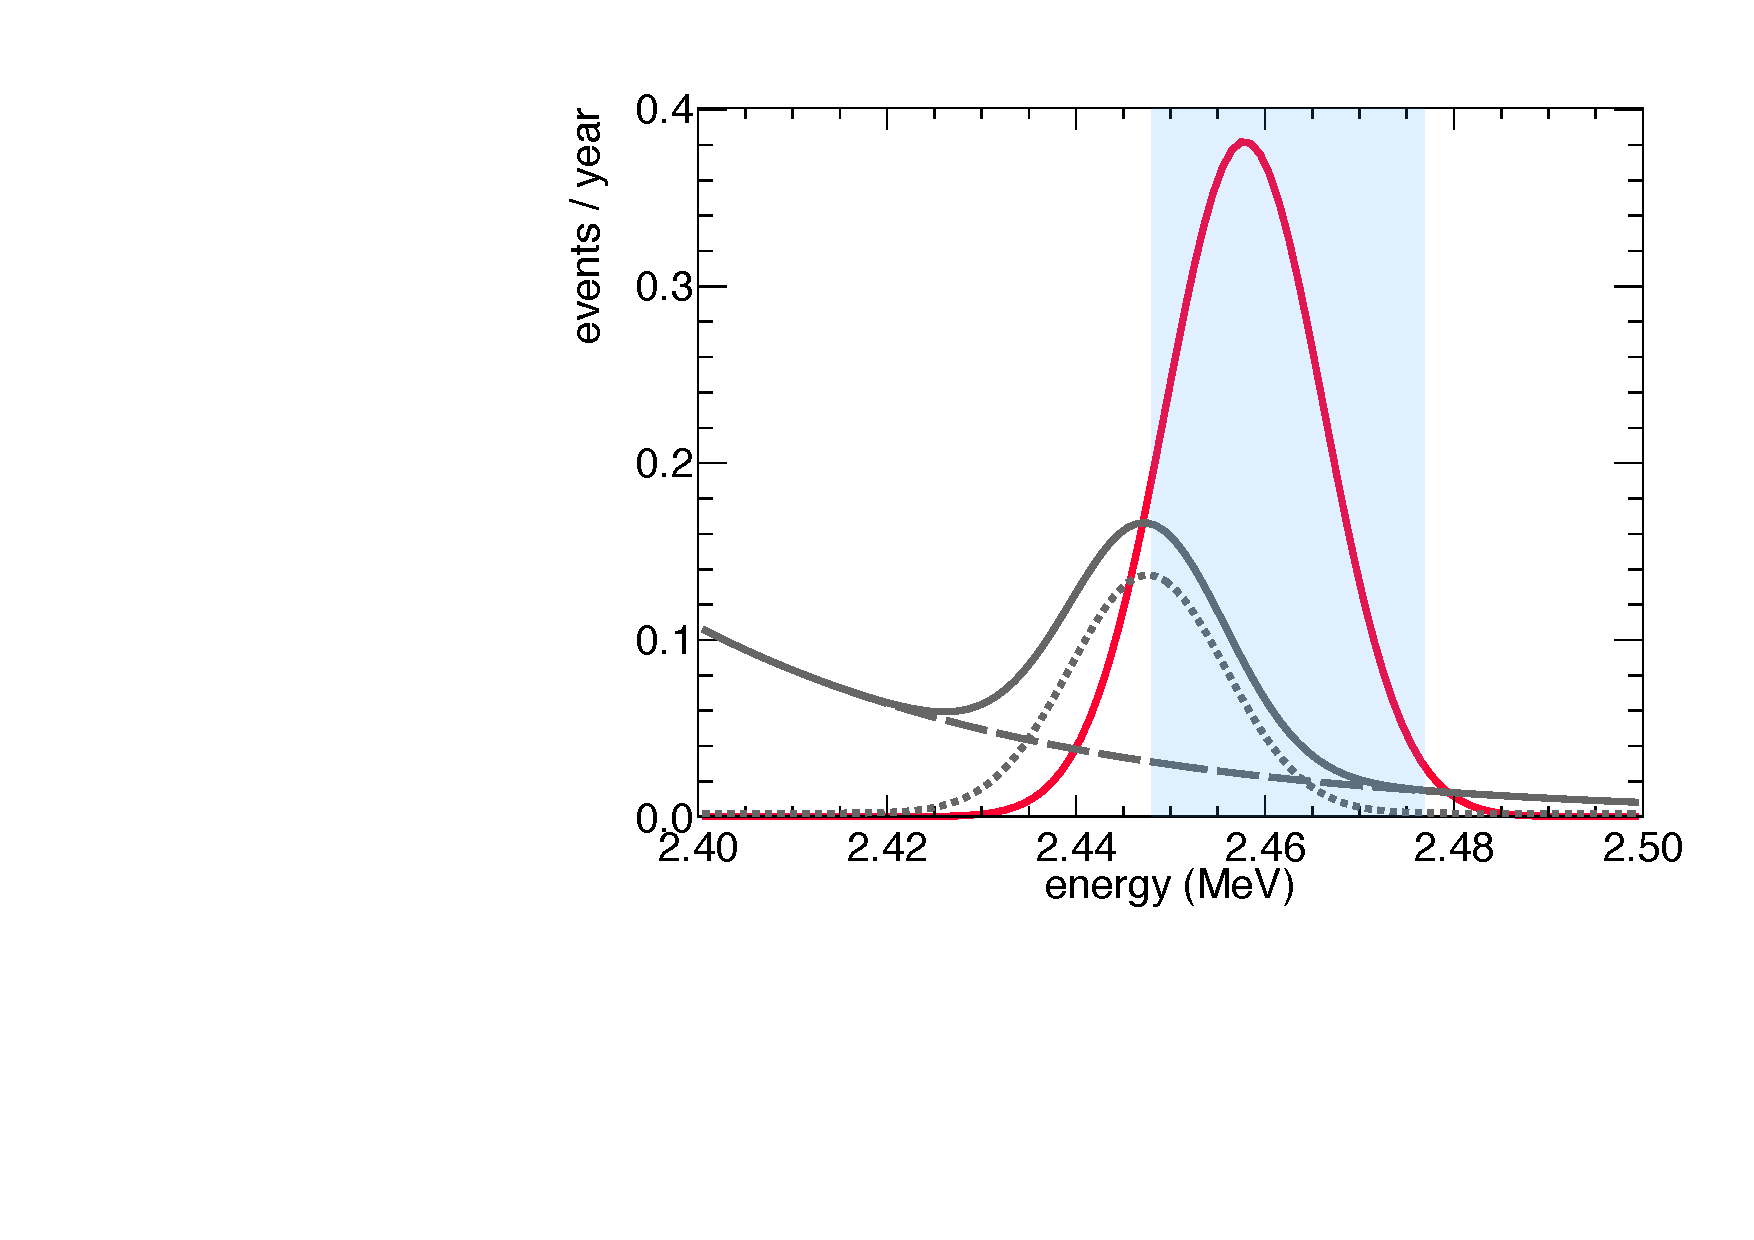
\includegraphics[width=0.9\textwidth]{img2/Next100ROI.pdf}
\caption{Energy spectra of signal (red, solid curve) and background (\Tl: grey, dashed distribution; \Bi: grey, dotted distribution; total: grey, solid distribution) in the region of interest (ROI) around \Qbb. The optimal ROI (the one that maximizes the ratio of the signal efficiency over the square root of the background rate) is indicated by the shaded, blue region. The signal strength represented here corresponds to a neutrino Majorana mass of 200 meV, while the backgrounds are scaled to their expected values in NEXT-100 ($6\times10^{-4}$~\ckky), assuming an exposure of 91~kg~yr.} \label{fig:ROI}
\end{figure}
%%%%%%%%%%


Table~\ref{tab:AcceptanceSelectionCriteria} summarizes the acceptances for signal and background of the selection criteria described above. The natural radioactive backgrounds, \TL\ and \BI, are suppressed by morel than 6 orders of magnitude, and the contribution of \bbtnu-decay to the background rate is completely negligible. The cuts yield a signal efficiency of 28\%. Note, however, that approximately half of the events are lost already in the first selection cut: 88\% of the events are contained within the fiducial volume of the detector, 71\% have one single track, and 76\% of them have reconstructed energy above 2.4~MeV (the \bbonu\ spectrum has a tail extending to low energies composed of events with missing energy in the form of bremsstrahlung radiation).

%%%%%%%%%%
\begin{table}[!]
\centering
\begin{tabular}{l c l l l}
\toprule
%
Selection criterion & \multicolumn{1}{c}{\bbonu} & \multicolumn{1}{c}{\bbtnu} & \multicolumn{1}{c}{\Tl} & \multicolumn{1}{c}{\Bi} \\ \midrule
Fiducial, single track & \multirow{2}{*}{0.4759} & \multirow{2}{*}{$8.06\times10^{-9}$} & \multirow{2}{*}{$2.83\times10^{-5}$} & \multirow{2}{*}{$1.04\times10^{-5}$} \\
$E\in[2.4, 2.5]~\mathrm{MeV}$ \\ \addlinespace
%
Track with 2 blobs & 0.6851 & 0.6851 & 0.1141 & 0.105 \\ \addlinespace
%
Energy ROI & 0.8661 & $3.89\times10^{-5}$ & 0.150 & 0.457 \\ \addlinespace
%
\emph{Total} & 0.2824 & $2.15\times10^{-13}$ & $4.9\times10^{-7}$ & $4.9\times10^{-7}$ \\
\bottomrule
\end{tabular}
\caption{Acceptance of the selection criteria for \bbonu-decay events described in the text. The values for \Tl\ and \Bi\ correspond to one of the dominant sources of background in the detector.} \label{tab:AcceptanceSelectionCriteria}
\end{table}
%%%%%%%%%%
